\documentclass[10.5pt
%,draft
]{article}

\usepackage{ctex}
\usepackage{graphicx}
\usepackage{amsmath}
\usepackage{physics}
\usepackage{geometry}
\usepackage{natbib}
\usepackage{subcaption}

\renewcommand{\refname}{参考文献}
\renewcommand{\figurename}{图}
\renewcommand{\abstractname}{摘要}

\def\due{2023 年 4 月 7 日周五 8:40}
\def\Term{2023 年春季}
\def\Course{磁流体力学的数值模拟方法}

\begin{document}

\title{行波方程和 Burgers 方程的数值计算 \\
  第 2 次作业\footnote{\Term\Course}}

\author{徐均益\footnote{ID: SA22168021 Email: jyxu@mail.ustc.edu.cn}
  \and
  余航\footnote{ID: SA22168021 Email: yh131996@mail.ustc.edu.cn}
  \and
  陈宇韬\footnote{ID: SA22214014 Email: chenyut@mail.ustc.edu.cn}
}

\date{%
\scriptsize%
%CAS Key Laboratory for Basic Plasma Physics, School of Earth and Space Sciences,
%\\
%University of Science and Technology of China, Hefei, Anhui 230026, China
中国科学技术大学地球与空间科学学院, 合肥 230026
中国科学技术大学物质科学研究院等离子所, 合肥 230026
%
}


\maketitle

\begin{abstract}
课程《磁流体力学的数值模拟方法》的第二次作业,讨论一维单一变量双曲型方程,其中包括行波方程和 $Burgers$ 方程的有限差分数值解法,
结合分析讨论几种常用的差分格式的特点. 如迎风格式,$Lax-Wendroff$格式,已经斜率补偿的限制器模式。行波方程与 $Burgers$ 方程采用了两种不同的初始输入,其中行波方程主要讨论在传播同样的距离条件下不同方法的耗散程度;而 $Burgers$ 方程则采用行波方程中比较好的斜率补偿限制器的方法,对波形在传播的不同时刻进行观测,同时与理论值进行对比分析结果。
\end{abstract}

\section{引言与背景}
波动是流体运动的一种重要形式,一般指的是在一个已经处于平衡态的流体体系中,收到小扰动时,其对应物理量的扰动随着时间在空间上进行传播,其在时间上与空间上具有双重周期性。其中对于线性一维的波动方程
\begin{align}
& \frac{\partial u^2}{\partial^2 t} - a^2 \frac{\partial u^2}{\partial x^2} = 0
\label{EqnCon}
\end{align}
可以变形分解为两个方向的行波解。
\begin{align}
    & \left \frac{\partial }{\partial t} + a \frac{\partial }{\partial x} \right \left \frac{\partial }{\partial t} - a \frac{\partial }{\partial x} \right= 0
\label{EqnCon}
\end{align}
本次研究对象为其中正向传播的行波方程。

另外流体力学中也会存在一些典型的非线性波动现象,如激波等等。在激波发生时,会在上游流体与下有流体之间出现一层流体状态量极具空间变化的过程。为了模拟激波的生成,我们采用了简单的非线性$Burgers$方程
\begin{align}
\frac{\partial u}{\partial t} + u \frac{\partial u}{\partial x} = 0, \label{EqnBurgers}
\end{align}
通过选用具体的某些初始函数的形状,通过模拟实验观察激波的生成。

本次实验重点在于以上述两个波动方程为基础,通过对比不同的模拟数值方法与参数,来分析对比不同的数值方法的特点与优劣,其中包括迎风格式,$LaxWendroff$高精度格式,以及采用斜率修正的限制器格式。

\section{实验方法以及对应的理论部分}
\subsection{行波方程的理论和方法}
行波方程
\begin{align}
& \frac{\partial u}{\partial t} + \frac{\partial u}{\partial x} = 0,
\label{EqnCon}
\end{align}
\subsection{$Burgers$方程的理论和方法}
$Burgers$方程
\begin{align}
\frac{\partial u}{\partial t} + u \frac{\partial u}{\partial x} = 0, \label{EqnBurgers}
\end{align}


\section{实验结果及解释描述}
\subsection{行波方程数值模拟部分}
考察方程
\begin{align}
& \frac{\partial u}{\partial t} + \frac{\partial u}{\partial x} = 0,
\label{EqnCon}
\end{align}
在初值条件
\begin{align}
& u|_{t=0} = \left\{\begin{array}{ll} 0.0, & x < -0.4, \\
1.0 - |x + 0.3| / 0.1, & -0.4 \le x < -0.2, \\
0.0, & -0.2 \le x < -0.1, \\
1.0 , & -0.1 \le x < 0.0, \\
0.0, & x \ge 0.0
\end{array}\right.
\end{align}
下的数值解. 通过有限差分格式, 如迎风格式
\begin{equation}
u_j^{n+1} = u^n - \frac{\Delta t}{\Delta x} (u_j^n - u_{j-1}^n), \label{EqnUpwind}
\end{equation}
Lax-Wendroff 格式
\begin{align}
	u_j^{n+1} 
	=&
	u_j^{n} 
	-
	\frac{a \Delta t}{ 2 \Delta x } (  	u_{j+1}^{n} - u_{j-1}^{n} ) \\
	&+ \frac{1}{2} \left( \frac{a \Delta t}{ \Delta x } \right)^2 (  	u_{j+1}^{n}- 2 u_j^n + u_{j-1}^{n} )
\end{align}

Limiters 
\begin{equation}
\begin{aligned}
u_i^{n+1}= & \frac{a \Delta t}{\Delta x}\left(u_{i-1}^n+\frac{1}{2}(\Delta x-a \Delta t) \sigma_{i-1}^n\right)+ \\
& \left(1-\frac{a \Delta t}{\Delta x}\right)\left(u_i^n-\frac{1}{2} a \Delta t \sigma_i^n\right) \\
= & u_i^n-\frac{a \Delta t}{\Delta x}\left(u_i^n-u_{i-1}^n\right)-\frac{1}{2} \frac{a \Delta t}{\Delta x}(\Delta x-a \Delta t)\left(\sigma_i^n-\sigma_{i-1}^n\right)
\end{aligned}
\end{equation}
其中
\begin{equation}
	\sigma_i^n = \verb|minmod| ( \frac{u_i^n - u_{i-1}^{n}}{ \Delta x }, \frac{u_{i+1}^n - u_{i}^{n}}{ \Delta x } )
\end{equation}
\begin{equation}
	\verb|minmod|(a, b) = 
	\begin{cases}
		a, \qif |a| < |b| \qand ab > 0\\
		b, \qif |a| > |b| \qand ab > 0\\
		0, \qif ab \leq 0.
	\end{cases}
\end{equation}


讨论该方程的物理解和差分格式数值解的特性. 要求
\begin{enumerate}
\item
  设计和编写程序进行数值计算试验, 试验和比较不同格式, 不同网格密度, 不同时间步长的计算结果.
网格密度为 428,时间步长 Courant 系数 ($C = \Delta t / \Delta x$) 为 0.05, 0.5, 0.95, 1.0
\item
  以图形来表示数值解的发展和变化. 和解析解比较, 分析数值解在间断附近的特性, 如速度, 过渡区宽度等.
\item
  试验一下不稳定差分格式 (如空间前向差分的 Euler 格式) 的数值计算过程, 说明所得到的结果.
\item
  如果可能, 分析数值耗散和色散效应.
\end{enumerate}

作为参考, 图~\ref{LinearW} 是方程~(\ref{LinearW}) 的不同格式, 不同 Courant 系数 ($C = \Delta t / \Delta x$), 在 $t = 0.5$ 的计算结果. 其中,
实线是精确解, 点线表示初态值, 虚线是数值计算结果, 而圆圈是具体网格 (单元) 上的数据. 
\begin{figure} 
\centering
\begin{subfigure}{.48\linewidth}
	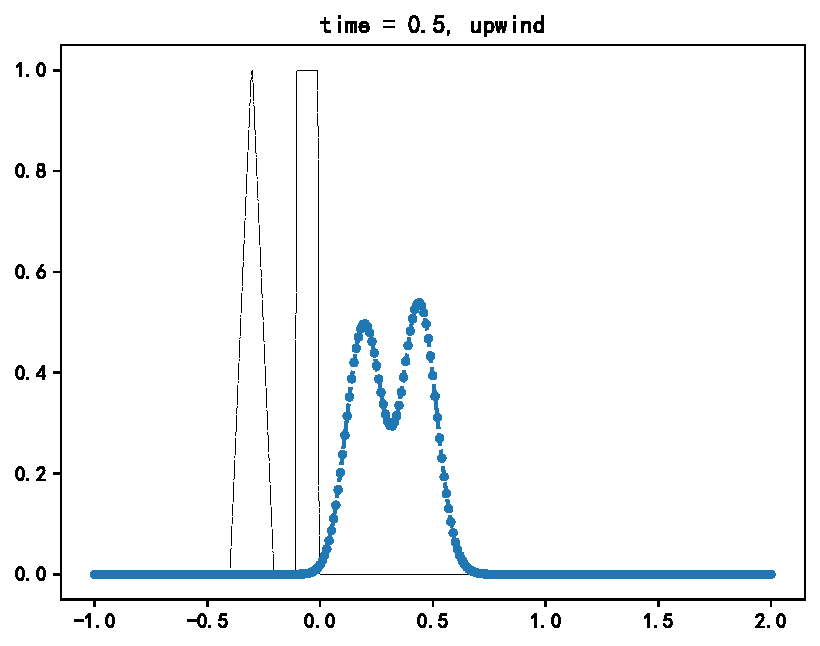
\includegraphics[width=\textwidth]{figures/problem1_upwind0.05.pdf}
  \caption{}
  \label{fig:problem1-1}
\end{subfigure}
\hfill
\begin{subfigure}{.48\linewidth}
  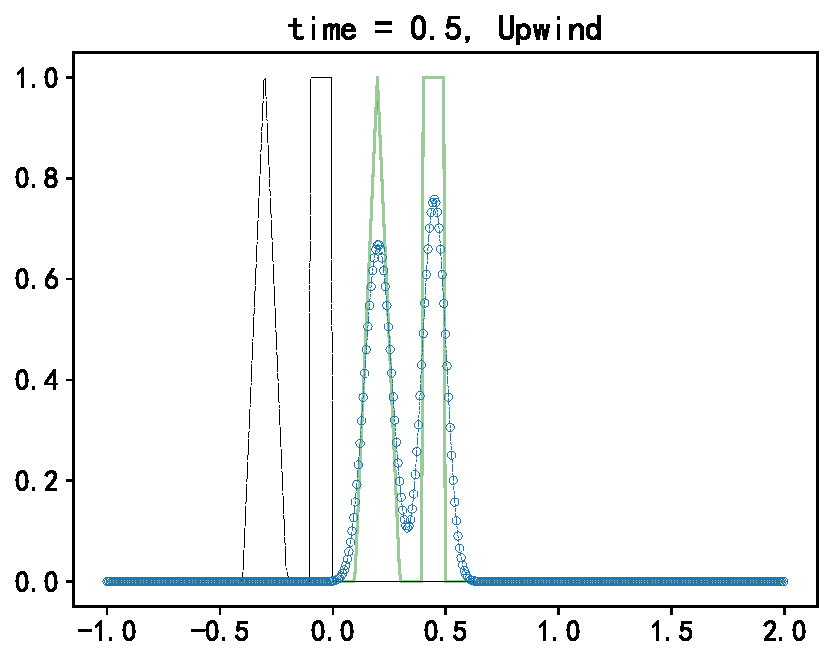
\includegraphics[width=\textwidth]{figures/problem1_upwind0.5.pdf} % second figure itself
  \caption{}
  \label{fig:problem1-2}
\end{subfigure}
\begin{subfigure}{.48\linewidth}
  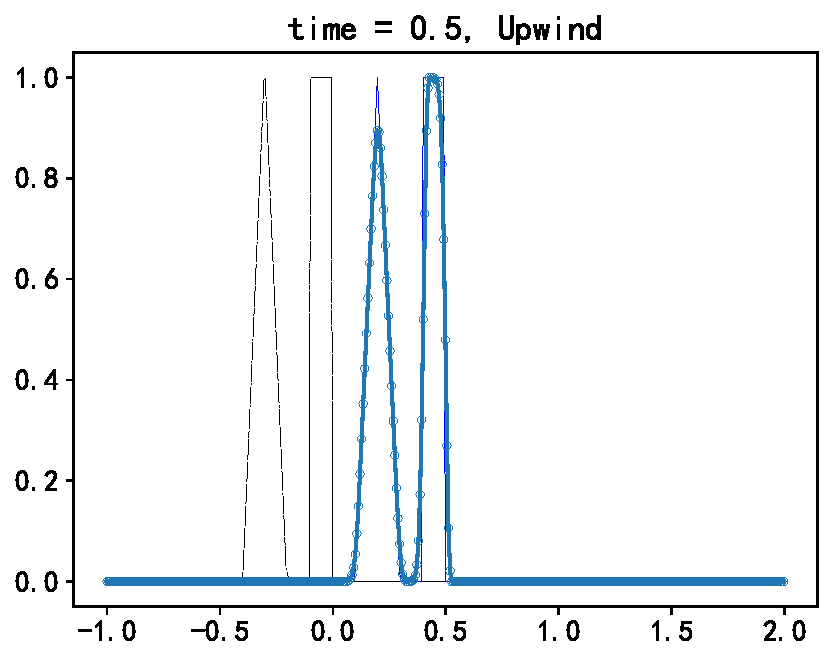
\includegraphics[width=\textwidth]{figures/problem1_upwind0.95.pdf}
  \caption{}
  \label{fig:problem1-3}
\end{subfigure}
\hfill
\begin{subfigure}{.48\linewidth}
  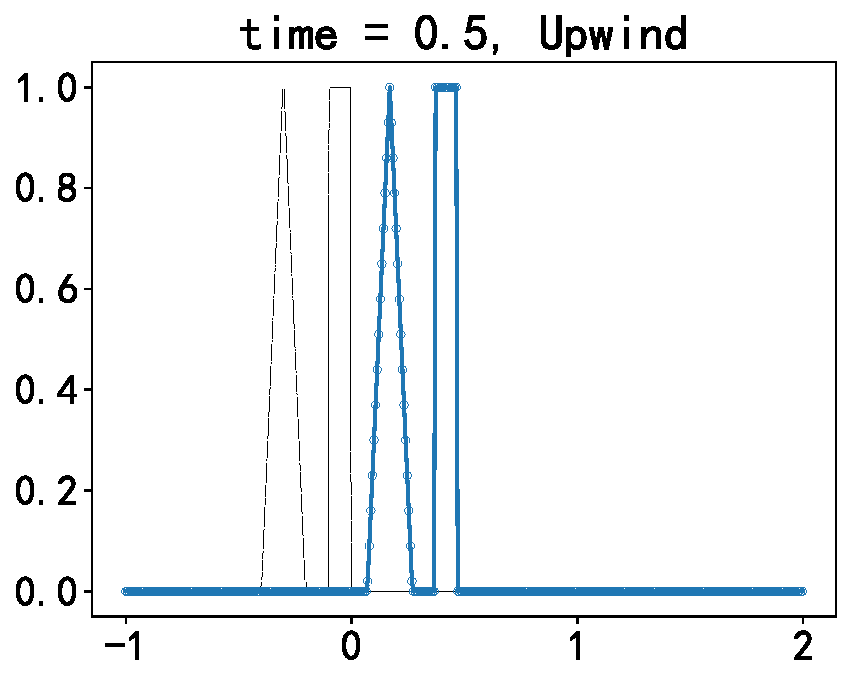
\includegraphics[width=\textwidth]{figures/problem1_upwind1.0.pdf}
  \caption{}
  \label{fig:problem1-4}
\end{subfigure}
\begin{subfigure}{.48\linewidth}
  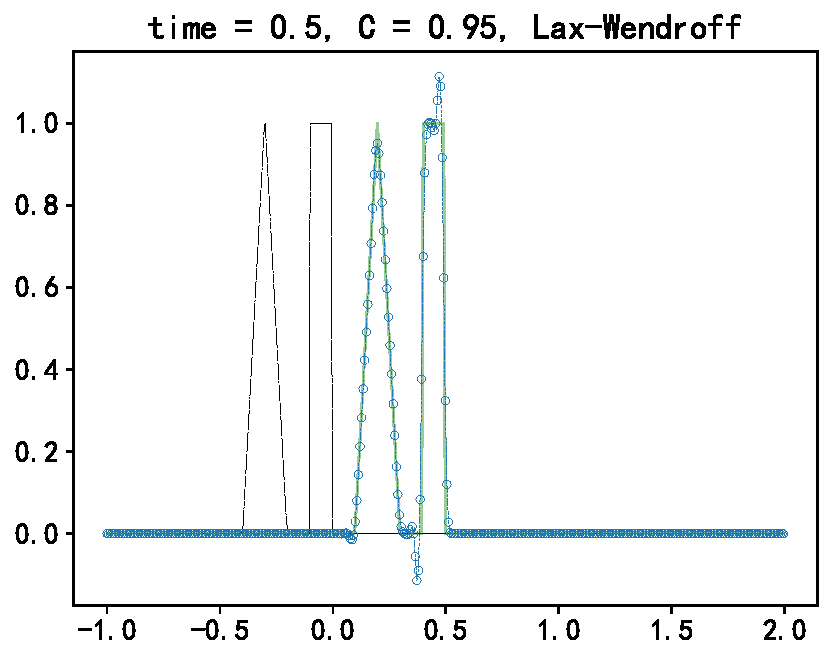
\includegraphics[width=\textwidth]{figures/problem1_lax_wendroff0.95.pdf}
  \caption{}
  \label{fig:problem1-5}
\end{subfigure}
\hfill
\begin{subfigure}{.48\linewidth}
  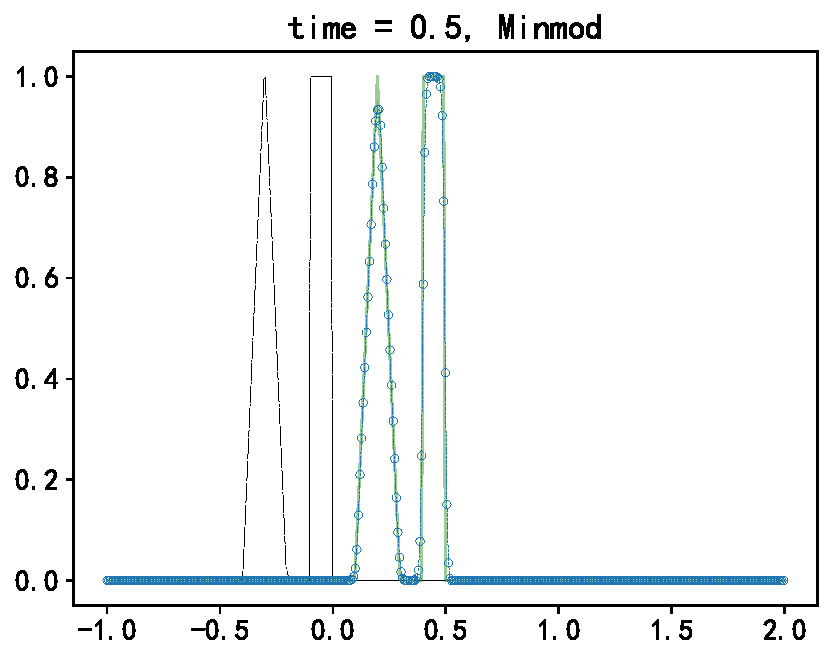
\includegraphics[width=\textwidth]{figures/problem1_limiter0.95.pdf}
  \caption{}
  \label{fig:problem1-6}
\end{subfigure}
\caption{方程~(\ref{EqnCon}) 在 $t=0.5$ 时刻的解. 其中虚线表示数值迎风格式的计算结果, 线上的圆圈表示具体网格上的数据. 同一时刻的精确解用实线表示. 作为对照,
  初始时刻的值以点线表示, 坐标网格总数为 517. (a) 迎风格式, $C = 0.05$, (b)  迎风格式, $C = 0.50$, (c)  迎风格式, $C = 0.95$, (d) 迎风格式, $C = 1.0$,
  此时数值解与精确解完全相同, (e) Lax-Wendroff格式, $C=0.95$, 注意其中出现的色散 (上冲和下冲), (f) Minmod格式, $C=0.95$.} \label{LinearW}
  \label{fig:problem1}%
\end{figure}


\subsection{$Burgers$方程数值模拟部分}
考察方程
\begin{align}
\frac{\partial u}{\partial t} + u \frac{\partial u}{\partial x} = 0, \label{EqnBurgers}
\end{align}
\begin{equation}
u_j^{n+1} = u^n - \frac{\Delta t}{\Delta x} \left( \frac{1}{2} (u_j^n)^2 - \frac{1}{2} (u_{j-1}^n)^2\right), \label{EqnUpwind}
\end{equation}

Limiters 
\begin{equation}
\begin{aligned}
u_i^{n+1}=&
  u_i^n-\frac{a \Delta t}{\Delta x}\left( \frac{1}{2} (u_i^n)^2- \frac{1}{2} (u_{i-1}^n)^2 \right)-
 &\frac{1}{2} \frac{a \Delta t}{\Delta x}(\Delta x-a \Delta t)\left(\sigma_i^n-\sigma_{i-1}^n\right)
\end{aligned}
\end{equation}
其中
\begin{equation}
	\sigma_i^n = \verb|minmod| \left( \frac{ \frac{1}{2} (u_i^n)^2 - \frac{1}{2} (u_{i-1}^{n})^2 }{ \Delta x }, \frac{ \frac{1}{2} (u_{i+1}^n)^2 - \frac{1}{2} (u_{i}^{n})^2}{ \Delta x } \right)
\end{equation}
\begin{equation}
	\verb|minmod|(a, b) = 
	\begin{cases}
		a, \qif |a| < |b| \qand ab > 0\\
		b, \qif |a| > |b| \qand ab > 0\\
		0, \qif ab \leq 0.
	\end{cases}
\end{equation}
在初值为
\begin{align}
u|_{t=0} = \left\{\begin{array}{ll} 1.8, & x < -0.8,
\\
1.4 + 0.4 \cos\left[2 \pi (x + 0.8) \right], & -0.8 \le x < -0.3,
\\
1.0, & -0.3 \le x < 0.0,
\\
1.8, & x \ge 0.0
\end{array} \right.
\end{align}
时的数值解. 设计一到多个差分格式, 分析数值计算结果并进行讨论. 要求
\begin{enumerate}
\item
  设计和编写程序进行数值计算试验.
\item
  以图形来表示数值解的发展和变化.
\item
  可能的话, 分析数值耗散和色散效应 (间断的宽度, 传播速度, 产生的数值解振荡等).
\end{enumerate}

图~\ref{BurgersW} 是方程~(\ref{EqnBurgers}) 的迎风格式在时间 $t = 0.25$, $0.5$, $0.75$, 和 $1.0$ 的计算结果, 其中 Courant 系数取 0.95,
即 $\Delta t = 0.95 \frac{\Delta x}{\max(u)}$.

\begin{figure} 
\centering
\begin{subfigure}{.9\linewidth}
  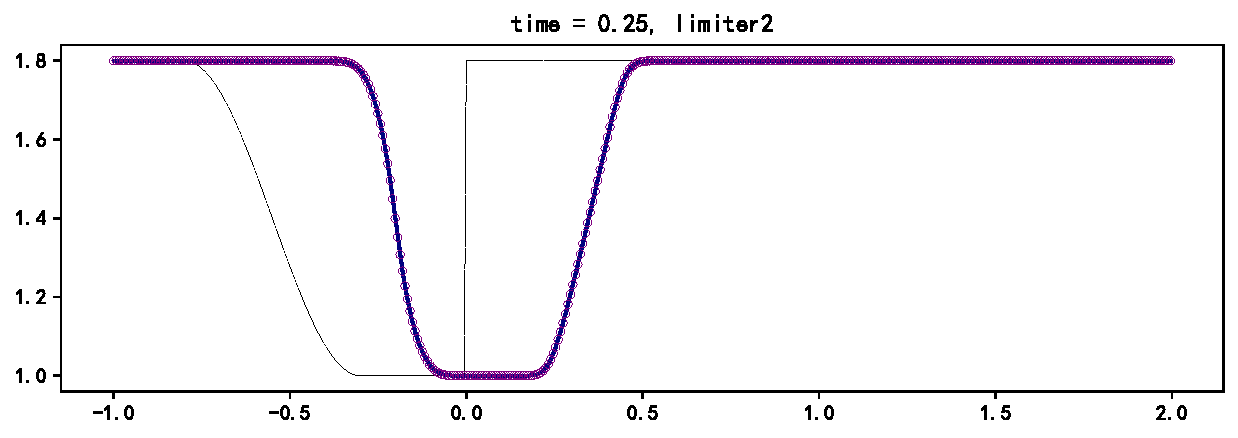
\includegraphics[width=\textwidth]{figures/problem2_limiter20.25.pdf} % first figure itself
  \label{fig:problem2-1}
\end{subfigure}
\begin{subfigure}{.9\linewidth}
  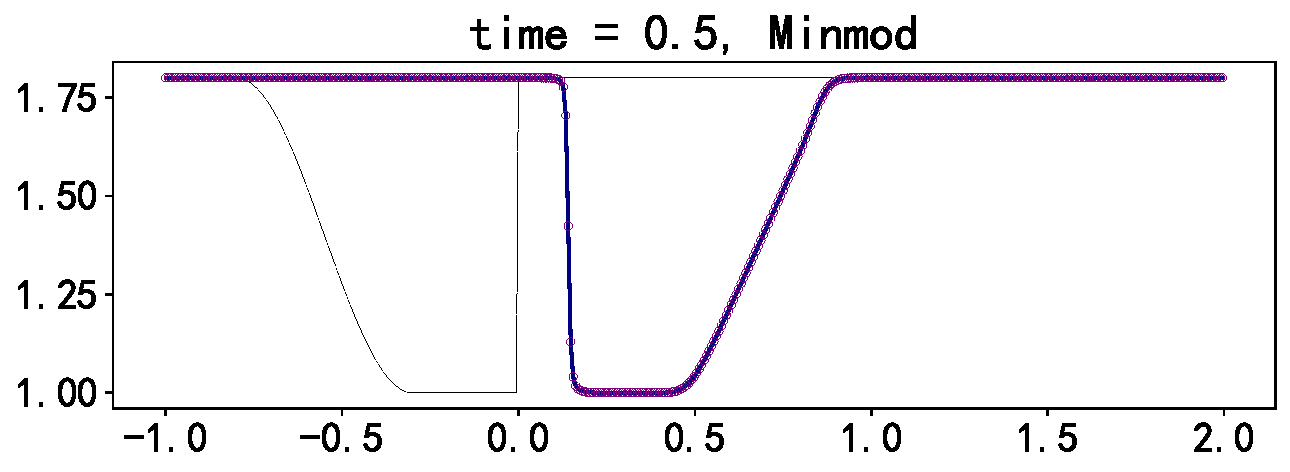
\includegraphics[width=\textwidth]{figures/problem2_limiter20.5.pdf} % first figure itself
  \label{fig:problem2-2}
\end{subfigure}
\begin{subfigure}{.9\linewidth}
  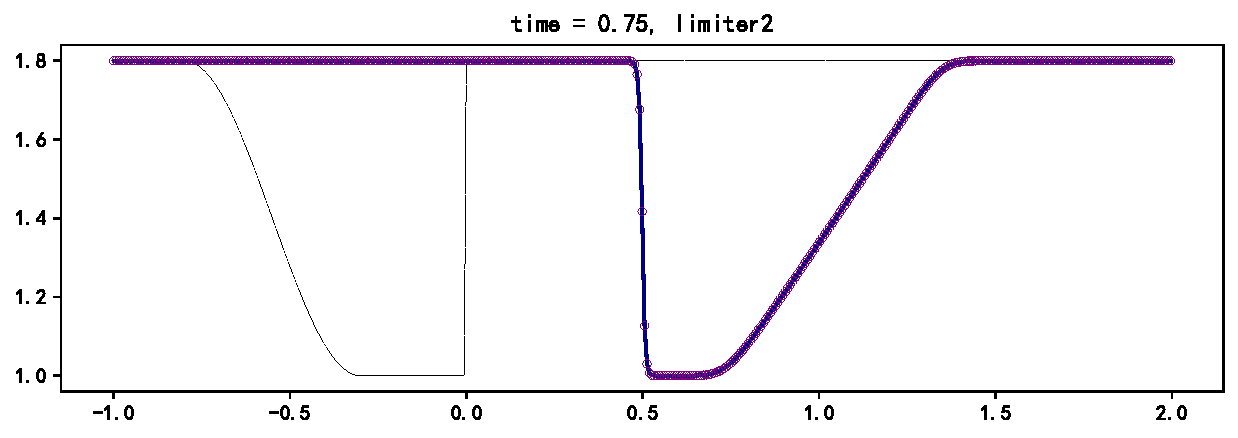
\includegraphics[width=\textwidth]{figures/problem2_limiter20.75.pdf} % first figure itself
  \label{fig:problem2-3}
\end{subfigure}
\begin{subfigure}{.9\linewidth}
  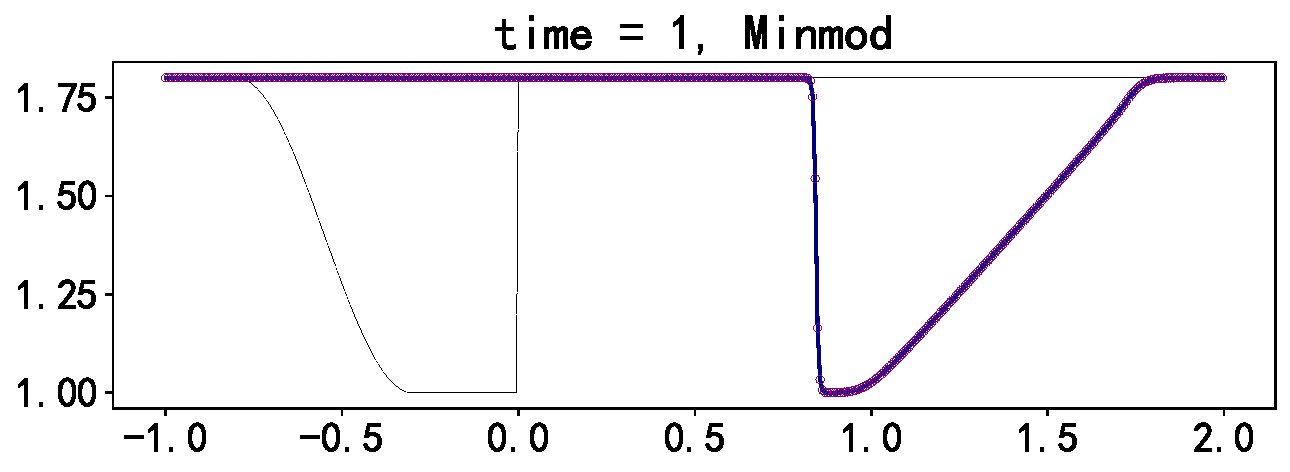
\includegraphics[width=\textwidth]{figures/problem2_limiter21.pdf} % first figure itself
  \label{fig:problem2-4}
\end{subfigure}
\caption{%
  方程~(\ref{EqnBurgers}) 的 Minmode 格式计算结果, 采用了 428 个网格, Courant 系数 $C$ 取为 0.2. 虚线表示数值格式的计算结果, 其中上面的圆圈表示具体的数据;
  解析解用实线表示, 初始时刻的值以点线表示. (a) $t=0.25$, (b) $t=0.5$, (c) $t=0.75$, (d) $t=1.0$.
}
  \label{fig:problem2-summary}%
\end{figure}

\section{分工说明}

郑惠南提供了最初的报告文本, 由数值计算结果生成的图形文件. 高新亮对整个文档结构, 规范, 文件清单进行了检查, 确认.

\section{附件}

\begin{enumerate}
\item
assign2.tex -- 本报告的 \LaTeX 文件
\item
assign2.pdf -- 本报告的 PDF (Portable Document Format) 输出文件
\item
References.bib -- 文献文件
\item
LinearW517005.eps -- 行波方程~(\ref{EqnCon}) 的数值计算结果, 对应图~\ref{LinearW}(a)
\item
LinearW517050.eps -- 行波方程~(\ref{EqnCon}) 的数值计算结果, 对应图~\ref{LinearW}(b)
\item
LinearW517095.eps -- 行波方程~(\ref{EqnCon}) 的数值计算结果, 对应图~\ref{LinearW}(c)
\item
LinearW517100.eps -- 行波方程~(\ref{EqnCon}) 的数值计算结果, 对应图~\ref{LinearW}(d)
\item
LinearWLW517095.eps -- 行波方程~(\ref{EqnCon}) 的数值计算结果, 对应图~\ref{LinearW}(e)
\item
LinearWMM517095.eps - 行波方程~(\ref{EqnCon}) 的数值计算结果, 对应图~\ref{LinearW}(f)
\item
Burgers025.eps -- Burgers方程~(\ref{EqnBurgers}) 的数值计算结果, 对应图~\ref{BurgersW}(a)
\item
Burgers050.eps -- Burgers方程~(\ref{EqnBurgers}) 的数值计算结果, 对应图~\ref{BurgersW}(b)
\item
Burgers075.eps -- Burgers方程~(\ref{EqnBurgers}) 的数值计算结果, 对应图~\ref{BurgersW}(c)
\item
Burgers100.eps -- Burgers方程~(\ref{EqnBurgers}) 的数值计算结果, 对应图~\ref{BurgersW}(d)
\end{enumerate}

\section*{项目作业的一些要点}
为了更好地帮助同学们完成项目作业, 现将一些注意的检查要点和评分标准 (括弧中的数字) 罗列如下,
\begin{itemize}
\item
期限 (20)
\item
完整性/报告/清单/分工 (10)
\item
报告源文件和 PDF 输出文件, 源程序 (10)
\item
图形文件 (10): PDF 或 EPS (Encapulated PostScript) 格式文件. 鉴于对软件的熟悉程度不同, 不再要求 PDF 格式的图形文件, EPS 格式文件也可接受.
\item
规范-语法 (10): 论文的写作规范, 如文献引用, 图/表, 叙述之间的逻辑关联, 等等.
\item
变量公式规范 (10)
\item
正确性 (10)
\item
其它 (5): 结构, 概念, 表达, 排版, 等等
\end{itemize}

\bibliographystyle{apalike}
\bibliography{References}

\end{document}
